\documentclass{article}
\usepackage{graphicx} % Required for inserting images
\usepackage{pgf}
\usepackage{lmodern}
\usepackage{import}
\usepackage{booktabs}
\usepackage{tabu}
\usepackage{float}
\usepackage[hidelinks]{hyperref}
\usepackage{amsmath}
\usepackage{amsfonts}
\usepackage[margin=1in]{geometry}
\usepackage{pythonhighlight}
\usepackage[toc]{appendix}
\usepackage{float}
\usepackage{placeins}

\setlength{\parskip}{1em}
\setlength{\parindent}{0em}

\begin{document}
\begin{titlepage}
    \begin{center}
        \vspace*{7cm}

        \Huge
        \textbf{Coupled Pendula}

        \vspace{0.5cm}
        \LARGE
        PHYS2113 - Classical Mechanics

        \vspace{1.5cm}

        \textbf{Toby Nguyen - z5416116}
    \end{center}
\end{titlepage}

\tableofcontents

\newpage

\section{Introduction}
The pendulum experiment is one of the most prominent experiments when it 
comes to the introduction of physics to students. The simple premise of a 
swinging object combined with the surprising result that the period of the 
swinging object is independent of its mass epitomises the beauty of physics 
and how it can sometimes defy human intuition. It is then our ability to 
conduct experiments to further our understanding of the world rather than 
our reliance on our own constructed beliefs.

Hookes' law is again one of the most prominent introductory physics type 
experiments as it demonstrates the necessity of mathematics when coupled 
(no pun intended) with experimentation. Observing a spring by itself is 
uninteresting as it is unlikely that any non-mathematically inclined person
would see that the force from a spring is directly proportional to its 
displacement. It is the mathematical formula of 

\begin{equation}
    F = -kx
\end{equation}

that enables physicists to understand the spring force and how oscillating
motions comes in more forms than just waves. One of the most common experiments
is to calculate the spring constant $k$. To do so, one must produce a linear
graph of a spring's displacement vertically and its mass. The trick is that 
when the spring is at rest, its spring force and the force due to gravity are
equal,

\begin{equation}
    \begin{split}
        F_g &= F_s \\
        mg &= -kx.
    \end{split}
\end{equation}

Rearranging gives

\begin{equation} \label{eqn:hk}
    x = -\frac{g}{k}m.
\end{equation}

Building on the pendulum experiment is the coupled pendula. It is similar 
to its predecessor in the sense that the simplicity of the experiment is kept
however upon analysis, unexpected results might occur. By connecting two 
pendulums by a spring, the periodic motion of one pendulum is now dependent
on the motion of the other one. The equations of motion are derived in 
\ref{eqn:derivation} along with definitions of constants.

We define $A$ as

\begin{equation}
    A = \sqrt{\frac{g}{L}}
\end{equation}

where g is the acceleration due to gravity and L is the length of the rod.

Similarly, $B$ is defined as

\begin{equation}
    B = \frac{l}{L}\sqrt{\frac{k}{m}}
\end{equation}

where l is the distance from the top of the rod to the spring, k is the spring
constant and m is the mass of the pendulums.

We can now describe our equations of motions for each mode the pendula are in. 
For the pendula being in phase, their equation of motion is given as

\begin{equation} \label{eqn:ip}
    \phi_1(t) = \phi_2(t) = \phi_{max}\cos{(At)}
\end{equation}

where $\phi$ represents the function of angular displacement of each pendula.

When the pendula are out of phase, $\phi_1(t)=-\phi_2(t)$,

\begin{equation} \label{eqn:op}
    \begin{split}
        \phi_1(t)&=\phi_{max}\cos{\left(\sqrt{A^2+2B^2}t\right)} \\
        \phi_2(t)&=-\phi_{max}\cos{\left(\sqrt{A^2+2B^2}t\right)}.
    \end{split}
\end{equation}

Lastly, when the pendulums are in beatmode, or where $\phi_1(0)=\phi_{max}$
and $\phi_2(0)=0$ or vice versa, their equations of motion is described as

\begin{equation} \label{eqn:bm1}
    \begin{split}
    \phi_1(t) &= \phi_{max}\cos{\left(\frac{\sqrt{A^2+2B^2}-A}{2}t\right)}
    \cos{\left(\frac{\sqrt{A^2+2B^2}+A}{2}t\right)}. \\
    \phi_2(t) &= -\phi_{max}\sin{\left(\frac{\sqrt{A^2+2B^2}-A}{2}t\right)}
    \sin{\left(\frac{\sqrt{A^2+2B^2}+A}{2}t\right)}.
    \end{split}
\end{equation}

This can be represented as

\begin{equation} \label{eqn:bm2}
    \begin{split}
        \phi_1(t) &= \frac{\phi_{max}}{2}\left[\cos{\left(
        \sqrt{A^2+2B^2}t\right)}+\cos{\left(A t\right)}\right]. \\
        \phi_2(t) &= \frac{\phi_{max}}{2}\left[\cos{\left(
        \sqrt{A^2+2B^2}t\right)}-\cos{\left(A t\right)}\right]. 
    \end{split}
\end{equation}

\section{Aim}
The aim of this experiment is to first calculate the spring constant, $k$.
Using this value, we want to compare experimental results of coupled pendula
to the theoretical models presented in Equations \ref{eqn:ip}, \ref{eqn:op}
and \ref{eqn:bm1} to verify the validity of those models. We also want to 
compare the oscillating motions of uncoupled and coupled pendula in different 
modes to observe the qualitative effects of coupling two pendula. Lastly, using
Fourier Transforms, we want to obtain an measurement for the frequency of each
mode for different heights of the spring and compare them to theoretical values.

\section{Method}
\subsection{Experimental Setup}
The first part of the experiment was to measure the spring constant. To do so,
the following setup displayed below in Figure \ref{fig:kexp}. 
\begin{figure}[H] 
    \centering
    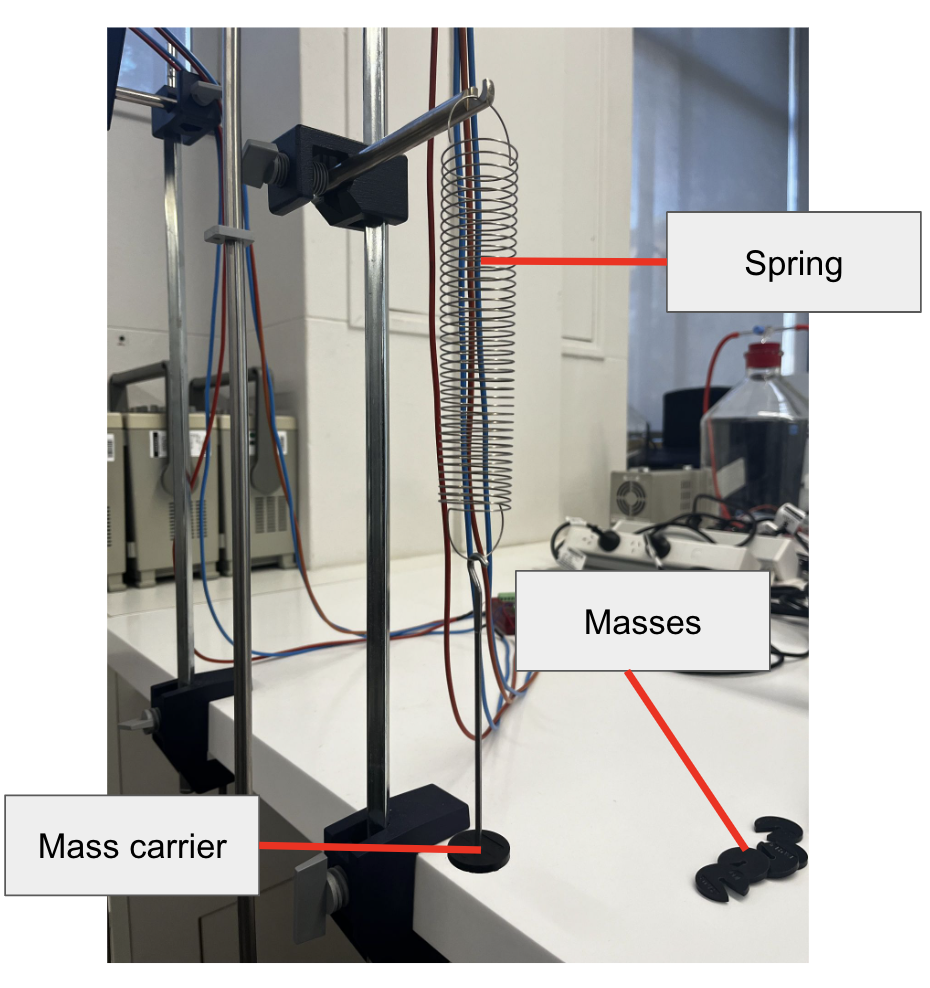
\includegraphics[width=0.5\textwidth]{setup1.png}
    \caption{Labelled picture of setup for calculating the spring constant.}
    \label{fig:kexp}
\end{figure}

The spring with no mass attached was initially measured to be 16cm long, indicating
this as the equilibrium length. The mass carrier, representing a 10g mass, was then 
attached and the length of the spring was measured again, once the mass was completely 
stationary, now displaced some $\Delta x$. As each 10g mass was added on, up to 50g, 
the length of the spring increased linearly. The graph of length of spring vs mass 
could then be plotted and its gradient used to find the constant $k$ using Equation 
\ref{eqn:hk}.

For the coupled pendula experiment, the setup in Figure \ref{fig:exp} was used. 
\begin{figure}[H] 
    \centering
    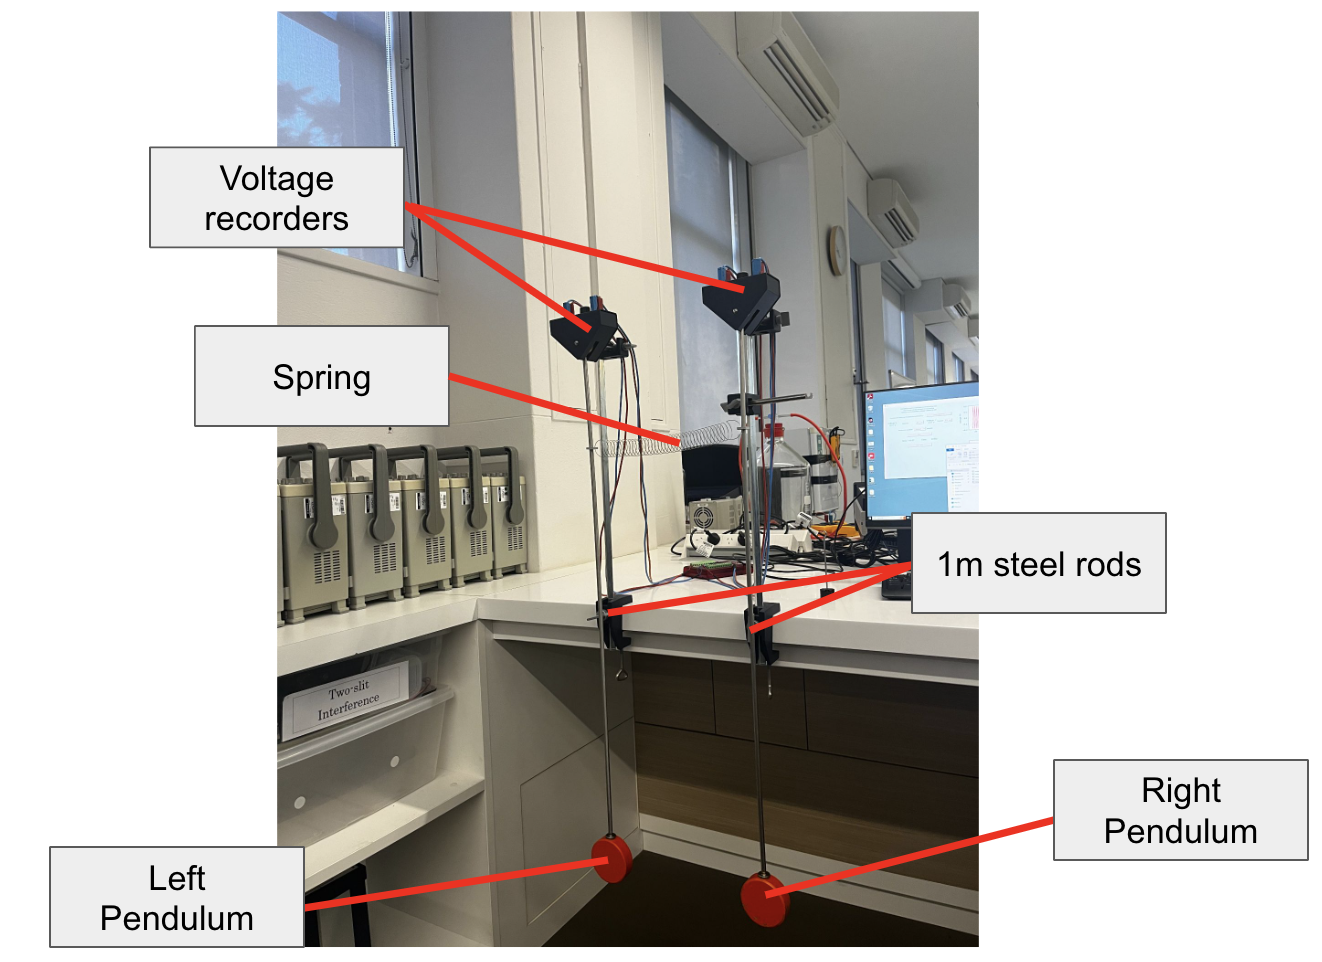
\includegraphics[width=0.8\textwidth]{setup2.png}
    \caption{Labelled picture of setup for coupled pendula.}
    \label{fig:exp}
\end{figure}

The pendula were then released in different modes. The voltage recorder records a 
max voltage of 20V and the corresponding pendulum has a maximum angular displacement
of 90$\deg$, indicating the angular displacement to voltage factor of 4.5$\deg$ per
1 volt. For the mode where the pendulas are in phase, both pendulums were released 
at a voltage recording of 0.2V, or 0.9$\deg$, maintaining the small angle assumption.
For both the cases where the pendula were out of phase and in beatmode, the pendula
and pendulum were released at 0.1V or 0.45$\deg$.

\subsection{Constants and Systematic Uncertainty} \label{eqn:sys}
In the previous section, the initial angular displacement was chosen for each mode.
This initial displacement represents $\phi_{max}$ and needs to be converted into radians
to utilise the small angle approximation. 

The resolution in the voltmeter was 0.01V indicating an absolute uncertainty of $\pm$0.005V.
This leads to a percentage uncertainty of 2.5\% for the inphase pendula and 5\% for the other
two modes.

The initial displacement for the pendula in phase is then
\begin{equation}
    \phi_{max} = 0.016 \pm 0.0004 \: \text{rad}.
\end{equation}

For the out of phase and beatmode modes, 

\begin{equation}
    \phi_{max} = 0.0079 \pm 0.0004 \: \text{rad}.
\end{equation}

From the PHYWE operating instructions page, the length fo the pendulum is said to be 1 m 
$\pm$ 2 cm, this value will be used as the masses were at the lowest point of the rod. The
percentage uncertainty contribution is then 2\%.

The mass of the system is a little bit more tricky to consider. In Appendix \ref{eqn:derivation},
we assumed the rods themselves were massless however physically that cannot be the case. We 
know that the mass of the system does not affect the period of the pendula for the single pendulum
experiment however the mass of the system in this case will affect the spring force. In the 
derivation we assumed that for the moment of inertia it was a point mass and so the mass was 
distributed all the way towards the bottom but in reality there is mass in the rod. According
to the PHYWE operating instructions page, the mass of the rods is approximately 100g and since 
measuring each component is unfeasible, the uncertainty contribution from the rod will be 5\% and
the total mass of the system, $m$, will be the sum of the pendulas and the rods so

\begin{equation}
    m = 1.1 \pm 0.06 \: \text{kg}.
\end{equation}

For lowercase l, the distance from the top of the rod to the spring, the only uncertainty comes 
from the ruler used. The smallest increment was 0.5cm so the uncertainty will be $\pm$0.25 cm.
The percentage uncertainty will then be taken as the average of the percentage uncertainties 
that came with each reading, l = 12.5cm, 25cm, 40cm, 50cm and 75cm.

\begin{equation}
    \sigma = \frac{1}{5}\sum_{i=12.5}^{75}\frac{0.25}{i}.
\end{equation}

Completing this sum, we will achieve a percentage uncertainty of
\begin{equation}
    \sigma \approx 1\%.
\end{equation}

The last constant $g$ can be assumed to have negligible uncertainty and a constant value of 
$-9.8ms^{-1}$.

We can now find the systematic uncertainty from adding each contribution 
in quadrature. For pendula in phase,

\begin{equation} \label{eqn:sys1}
    \begin{split}
        \sigma &= \sqrt{0.025^2+0.02^2+0.05^2+0.01^2} \\
        &= 0.06.
    \end{split}
\end{equation}

The systematic uncertainty for both the out of phase and pendula in beatmode
will be the same,

\begin{equation}
    \begin{split}
        \sigma &= \sqrt{0.05^2+0.02^2+0.05^2+0.01^2} \\
        &= 0.07.
    \end{split}
\end{equation}

\section{Results}
\begin{figure}
    \subsection{Spring Constant}
    \centering
    \scalebox{0.75}{\input{kcalc.pgf}}
    \caption{Line graph with a gradient of 0.31.}
    \label{fig:kgraph}
\end{figure}
\begin{figure}[p]
\subsection{Pendulas in phase}
    \centering
    \scalebox{0.52}{\input{inphase1.pgf}}
    \hspace{0.5cm}
    \scalebox{0.52}{\input{inphase2.pgf}}
  
    \vspace{0.5cm}
  
    \scalebox{0.52}{\input{inphase3.pgf}}
    \hspace{0.5cm}
    \scalebox{0.52}{\input{inphase4.pgf}}
  
    \vspace{0.5cm}
  
    \scalebox{0.52}{\input{inphase5.pgf}}
    \hspace{0.5cm}
    \scalebox{0.52}{\input{inphase6.pgf}}
  
    \caption{Plots of voltage vs time of varying spring heights, note 
    that the uncoupled pendula, l=0, has no correlation in their 
    pendula's motions.}
\end{figure}

\FloatBarrier

\begin{figure}[p]
\subsection{Pendulas in phase: Fourier Plots}
    \centering
    \scalebox{0.52}{\input{inphase1f.pgf}}
    \hspace{0.5cm}
    \scalebox{0.52}{\input{inphase2f.pgf}}
  
    \vspace{0.5cm}
  
    \scalebox{0.52}{\input{inphase3f.pgf}}
    \hspace{0.5cm}
    \scalebox{0.52}{\input{inphase4f.pgf}}
  
    \vspace{0.5cm}
  
    \scalebox{0.52}{\input{inphase5f.pgf}}
    \hspace{0.5cm}
    \scalebox{0.52}{\input{inphase6f.pgf}}
  
    \caption{Plots of voltage vs time of varying spring heights, note 
    that the uncoupled pendula, l=0, has no correlation in their 
    pendula's motions.}
\end{figure}

\FloatBarrier

\begin{figure}[p]
\subsection{Pendulas out of phase}
    \centering
    \scalebox{0.52}{\input{outphase1.pgf}}
    \hspace{0.5cm}
    \scalebox{0.52}{\input{outphase2.pgf}}
  
    \vspace{0.5cm}
  
    \scalebox{0.52}{\input{outphase3.pgf}}
    \hspace{0.5cm}
    \scalebox{0.52}{\input{outphase4.pgf}}
  
    \vspace{0.5cm}
  
    \scalebox{0.52}{\input{outphase5.pgf}}
    \hspace{0.5cm}
    \scalebox{0.52}{\input{outphase6.pgf}}
  
    \caption{Plots of voltage vs time of varying spring heights, note 
    that the uncoupled pendula, l=0, has no correlation in their 
    pendula's motions.}
\end{figure}

\FloatBarrier

\begin{figure}[p]
\subsection{Pendulas out of phase: Fourier Plots}
    \centering
    \scalebox{0.52}{\input{outphase1f.pgf}}
    \hspace{0.5cm}
    \scalebox{0.52}{\input{outphase2f.pgf}}
  
    \vspace{0.5cm}
  
    \scalebox{0.52}{\input{outphase3f.pgf}}
    \hspace{0.5cm}
    \scalebox{0.52}{\input{outphase4f.pgf}}
  
    \vspace{0.5cm}
  
    \scalebox{0.52}{\input{outphase5f.pgf}}
    \hspace{0.5cm}
    \scalebox{0.52}{\input{outphase6f.pgf}}
  
    \caption{Plots of voltage vs time of varying spring heights, note 
    that the uncoupled pendula, l=0, has no correlation in their 
    pendula's motions.}
\end{figure}

\FloatBarrier

\begin{figure}[p]
\subsection{Pendulas in beatmode}
    \centering
    \scalebox{0.52}{\input{bmphase1.pgf}}
    \hspace{0.5cm}
    \scalebox{0.52}{\input{bmphase2.pgf}}
  
    \vspace{0.5cm}
  
    \scalebox{0.52}{\input{bmphase3.pgf}}
    \hspace{0.5cm}
    \scalebox{0.52}{\input{bmphase4.pgf}}
  
    \vspace{0.5cm}
  
    \scalebox{0.52}{\input{bmphase5.pgf}}
    \hspace{0.5cm}
    \scalebox{0.52}{\input{bmphase6.pgf}}
  
    \caption{Plots of voltage vs time of varying spring heights, note 
    that the uncoupled pendula, l=0, has no correlation in their 
    pendula's motions.}
\end{figure}

\FloatBarrier

\begin{figure}[p]
\subsection{Pendulas in beatmode: Fourier Plots}
    \centering
    \scalebox{0.52}{\input{bmphase1f.pgf}}
    \hspace{0.5cm}
    \scalebox{0.52}{\input{bmphase2f.pgf}}
  
    \vspace{0.5cm}
  
    \scalebox{0.52}{\input{bmphase3f.pgf}}
    \hspace{0.5cm}
    \scalebox{0.52}{\input{bmphase4f.pgf}}
  
    \vspace{0.5cm}
  
    \scalebox{0.52}{\input{bmphase5f.pgf}}
    \hspace{0.5cm}
    \scalebox{0.52}{\input{bmphase6f.pgf}}
  
    \caption{Plots of voltage vs time of varying spring heights, note 
    that the uncoupled pendula, l=0, has no correlation in their 
    pendula's motions.}
\end{figure}

\FloatBarrier

\section{Analysis}
\subsection{Spring constant}
From Figure \ref{fig:k}, we can read off the gradient as 3.14. 
Equating this value to the gradient found in the relationship
in Equation \ref{eqn:hk}, we can obtain the spring constant,

\begin{equation}
    \begin{split}
        0.31 &= -\frac{g}{k} \\
        k &= \frac{9.8}{3.14} \\
        &= 3.12.
    \end{split}
\end{equation}

Our aforementioned uncertainty for this measurement is driven 
by the uncertainty of the ruler used to measure the length. Using
the 1\% found in Section \ref{eqn:sys}, we obtain a final measurement
including a total uncertainty,

\begin{equation}
    k = 3.12 \pm 0.03.
\end{equation}

\subsection{Coupled Pendula: In Phase}

The following table contains the average frequency from 3-5 readings
along with a random uncertainty measurement calculated using the 
formula,

\begin{equation}
    \sigma_{stat} = \frac{max - min}{2}.
\end{equation}

This method of calculating statistical uncertainty was used rather
than the standard deviation due to the limited of data points obtained.

The theoretical value for frequency was obtained using Equations \ref{eqn:ip},

\begin{equation}
    \begin{split}
        \omega &= A = \sqrt{\frac{g}{L}} \\
        f_{theoretical} &= \frac{1}{2\pi}\sqrt{\frac{g}{L}} \\
        &= \frac{1}{2\pi}\sqrt{\frac{9.8}{1}} \\
        &= 0.5. 
    \end{split}
\end{equation}

Since the result does not depend on l, the theoretical value is the same for 
all l.

The total uncertainty was found by adding the statistical and systematic 
uncertainties in quadrature,

\begin{equation}
    \sigma_{total} = \sqrt{\sigma_{stat}^2+\sigma_{systematic}^2}.
\end{equation}

\begin{table} [H]
    \centering
    \begin{tabular} {c|c|c|c|c|c}
        l (cm) & Experimental Frequency (Hz) & $\sigma_{stat}$ & $\sigma_{total}$ & 
        Theoretical Frequency (Hz) & Error \\
        \hline
        0 & 0.51 & 0\% & 6\% & 0.50 & 2\% \\
        \hline 
        12.5 & 0.51 & 1\% & 6\% & 0.50 & 2\% \\
        \hline
        25 & 0.51 & 1\% & 6\% & 0.50 & 2\% \\
        \hline
        40 & 0.51 & 0\% & 6\% & 0.50 & 2\% \\
        \hline
        50 & 0.50 & 0\% & 6\% & 0.50 & 0\% \\
        \hline
        75 & 0.50 & 1\% & 6\% & 0.50 & 0\% 
    \end{tabular}
\end{table}

We find that for all values of l, the experimental results agree with the 
theoretical model.

\subsection{Coupled Pendula: Out of Phase}
Displaying the results in a similar table, however this time the theoretical 
frequency is found using Equation \ref{eqn:op}.

\begin{equation}
    \begin{split}
        \omega &= \sqrt{A^2+2B^2} \\
        f_{theoretical} &= \frac{1}{2\pi}\sqrt{\frac{g}{L}+2\frac{l^2k}{L^2m}} \\
        &= \frac{1}{2\pi}\sqrt{\frac{(9.81)}{(1)}+2\frac{l^2(3.12)}{(1)^2(1.1)}} \\
        &= \frac{1}{2\pi}\sqrt{9.81+\frac{312}{55}l^2}.
    \end{split}
\end{equation}

\begin{table} [H]
    \centering
    \begin{tabular} {c|c|c|c|c|c}
        l (cm) & Experimental Frequency (Hz) & $\sigma_{stat}$ & $\sigma_{total}$ & 
        Theoretical Frequency (Hz) & Error \\
        \hline
        0 & 0.51 & 0\% & 7\% & 0.50 & 2\% \\
        \hline 
        12.5 & 0.51 & 1\% & 7\% & 0.50 & 2\% \\
        \hline
        25 & 0.51 & 0\% & 7\% & 0.51 & 0\% \\
        \hline
        40 & 0.52 & 0\% & 7\% & 0.52 & 0\% \\
        \hline
        50 & 0.53 & 0\% & 7\% & 0.53 & 0\% \\
        \hline
        75 & 0.57 & 1\% & 7\% & 0.57 & 0\% 
    \end{tabular}
\end{table}

\subsection{Coupled Pendula: Beatmode}
From Equation \ref{eqn:bm2}, we can expect two peaks in our Fourier transforms as
there are two different trigonometric functions being added. One peak should have the 
frequency,

\begin{equation}
    \begin{split}
        f &= \frac{1}{2\pi}\sqrt{A^2+2B^2} \\
        &= \frac{1}{2\pi}\sqrt{9.81+\frac{312}{55}l^2}. 
    \end{split}
\end{equation}

i.e the frequency we found in the out of phase pendula experiment.

Simiarly, the second peak should have the frequency,

\begin{equation}
    \begin{split}
        f &= \frac{1}{2\pi}A \\
        &= 0.5.
    \end{split}
\end{equation}

This table will omit the uncertainties because there were less data points taken, meaning
statistical uncertainty is negligible and thus total uncertainty is driven by systematic
uncertainty which is found to be a constant 7\% for all readings. To replace these columns,
$f_1$ will indicate the first peak, on the left, and $f_2$ will indicate the second peak, 
on the right, or simply $f_1 < f_2$. All $f$ columns are in Hz.

\begin{table} [H]
    \centering
    \begin{tabular} {c|c|c|c|c|c|c}
        l (cm) & Experimental $f_1$ & Theoretical $f_1$ & Error & Experimental $f_2$ & 
        Theoretical $f_2$ & Error \\
        \hline
        0 & 0.51 & 0.50 & 2\% & - & 0.50 & -\\
        \hline 
        12.5 & 0.51 & 0.50 & 2\% & - & 0.50 & -\\
        \hline
        25 & 0.51 & 0.50 & 2\% & - & 0.51 & -\\
        \hline
        40 & 0.51 & 0.50 & 2\% & 0.53 & 0.52 & 2\%\\
        \hline
        50 & 0.51 & 0.50 & 2\% & 0.53 & 0.53 & 0\% \\
        \hline
        75 & 0.51 & 0.50 & 2\% & 0.57 & 0.57 & 0\%
    \end{tabular}
\end{table}

\section{Discussion}
Qualitatively comparing the results of the uncoupled pendula
and the coupled pendula, we can see that the movements of the 
uncoupled pendula are uncorrelated. We can see that for coupled 
pendula as the amplitude of one pendulum increases, the amplitude
of the other pendulum will decrease whereas both pendulum's 
amplitudes remain relatively unchanged in the case of coupled pendula, 
only damping due to friction.

For the pendula in phase, the theoretical model suggests that the
frequency is independent of the height at which the spring is attached.
This was found to be experimentally true mostly as for lengths 0cm, 
12.5cm, 25cm, 40cm, 50cm and 75cm, the experiment results obtained were
0.51 $\pm$ 0.03, 0.51 $\pm$ 0.03, 0.51 $\pm$ 0.03, 0.51 $\pm$ 0.03,
0.50 $\pm$ 0.03 and 0.50 $\pm$ 0.03. All of these results agree with 
the theoretical frequency of 0.50.

In the case that the pendula were out of phase, outside of the lengths
$l=0$ and $l=12.5cm$ which both resulted in an experimental value of 
0.51 $\pm$ 0.04 compared to their theoretical value of 0.50, the other 
lengths saw the experimental and theoretical frequency agree with each 
other. The experimental frequencies found for 25cm, 40cm, 50cm and 75cm 
were 0.51 $\pm$ 0.04, 0.52 $\pm$ 0.04, 0.53 $\pm$ 0.04 and 0.57 $\pm$
0.04, agreeing with their theoretical values of 0.51, 0.52, 0.53 and 
0.57 respectively.

Lastly, for the pendula in beatmode, two peaks were found experimentally 
for some lengths which was expected by the theoretical model. Technically 
speaking, there should be two peaks for all the lengths however for some
small l, i.e l < 40cm, we find that $B=\frac{l}{L}\sqrt{\frac{k}{m}}$ 
approaches 0 and so in Equation \ref{eqn:bm2}, for the first cosine 
function,

\begin{equation}
    \begin{split}
        \sqrt{A^2+2B^2} &\rightarrow \sqrt{A^2}\\
        &= A.
    \end{split}
\end{equation}

So Equation \ref{eqn:bm2} reduces down to Equation \ref{eqn:ip} for
small l.

The first peak which is represented by the second cosine function in
Equation \ref{eqn:bm2}, was experimentally found to be 0.51 $\pm$ 0.04 
for all lengths. This represents a constant 2\% error from the 
theoretical value of 0.50 for all lengths. Experimentally, the first
cosine function representing the second peak only showed itself for 
$l \geq 40 cm$ so for lengths 40cm, 50cm and 75cm, the experimental
value for that second peak was found to be 0.53 $\pm$ 0.04, 0.53 
$\pm$ 0.04 and 0.57 $\pm$ 0.04 which agrees with the theoretical 
values of 0.52, 0.53 and 0.57 respectively.

For all experimental values obtained in this experiment, they agreed
with their respective theoretical models. However, this experiment 
can be improved by reducing uncertainties. The largest component of
systematic uncertainty was the voltage resolution. This can be 
improved by increasing the amount of decimal places recorded, 
increasing the accuracy of the reading. Similarly, the uncertainty 
contribution from the mass of the system could be reduced by taking 
apart each component and weighing them individually. Furthermore, by
using a more accurate formula for the moment of inertia of the system
rather than assuming it to be a point mass.

\section{Conclusion}
The aim of the experiment was successfully tested and the theoretical 
models were validated in a confident manner.

\appendix
\section{Pre-work}
\subsection{Theory} \label{eqn:derivation}
The free body diagram with labelled forces is shown below in 
Figure \ref{fig:coupledpendula}.

\begin{figure} [H]
    \centering
    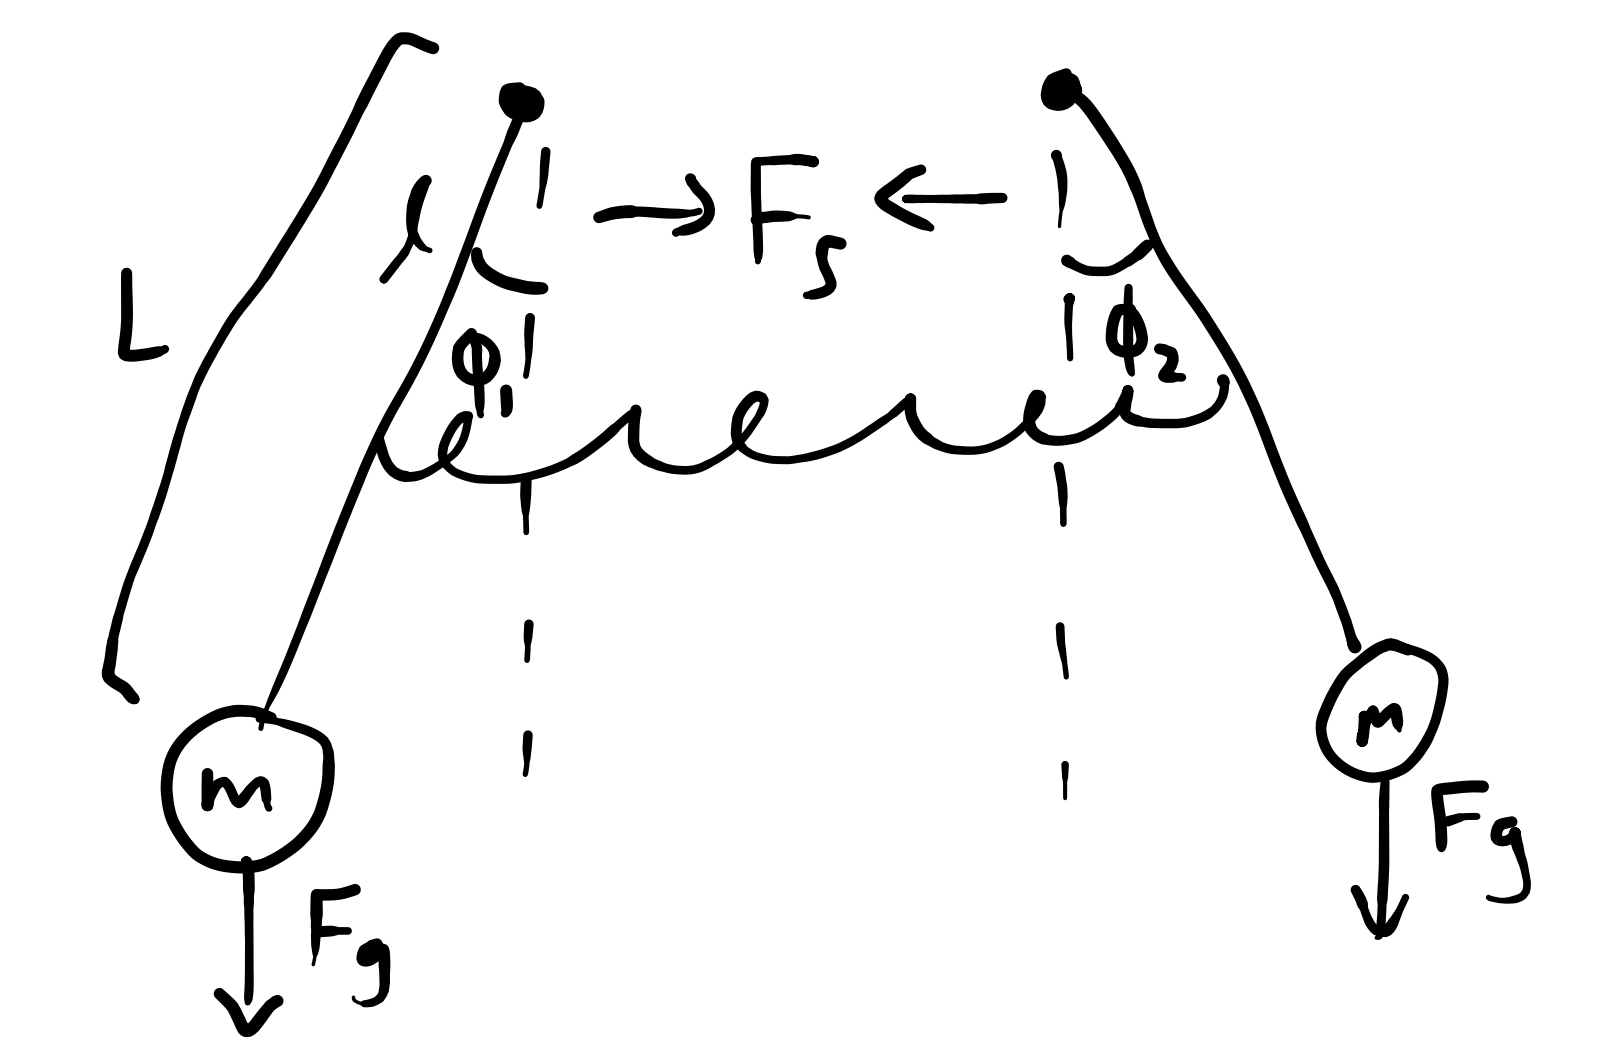
\includegraphics[width=0.5\textwidth]{coupledpendula.png}
    \caption{Free body diagram of coupled pendula. The two
    forces acting on the pendulums are the gravitational force, 
    $F_g$ and spring force, $F_s$.}
    \label{fig:coupledpendula}
\end{figure}

The net force of one of the pendulums is then,
\begin{equation} \label{eqn:netforce}
    F_{net} = F_g + F_s.
\end{equation}

The force due to gravity is simply $-mg$ and acts at an angle
$\phi_1$ to the rod, length L. For the spring force, consider
the free body diagram of two masses coupled by a spring shown
in Figure \ref{fig:twomass} below.

\begin{figure} [H]
    \centering
    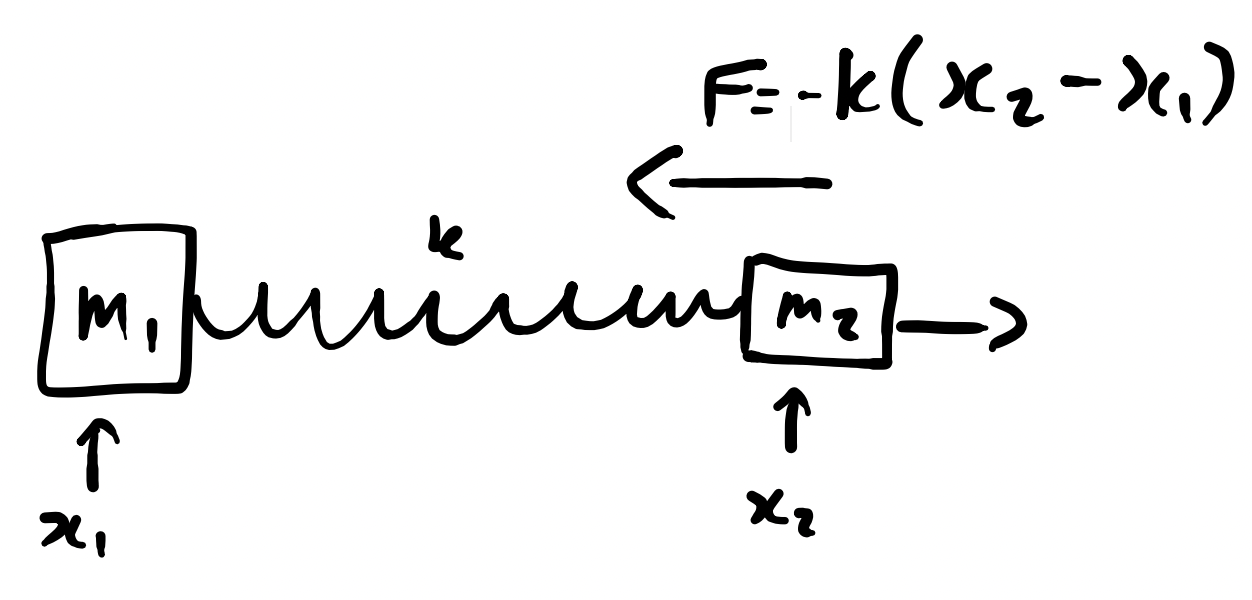
\includegraphics[width=0.5\textwidth]{twomass.png}
    \caption{Free body diagram of coupled masses.}
    \label{fig:twomass}
\end{figure}

Hooke's Law states that the restoring force on a spring is 
proportional to the displacement of a mass from its 
equilibrium length,
\begin{equation}
    F_s = -k\Delta x.
\end{equation}

In this case, there are two masses and they are coupled, 
meaning the displacement of one mass is influenced by the
position of the other mass. Hence the force on mass 1,

\begin{equation}
    F_s = -k(x_1 - x_2).
\end{equation}

Returning to our coupled pendula, the spring force, $F_s$
acting towards the spring when it is extended on the left
pendulum will be,

\begin{equation}
    F_s = -k(x_1 - x_2).
\end{equation}

The horizontal distances $x_1$ and $x_2$ can be rewritten in
terms of $\phi$,

\begin{equation}
    x = l\sin{\phi}.
\end{equation}

Therefore, the spring force on mass 1,
\begin{equation}
    F_s = -kl(\sin{\phi_2}-\sin{\phi_1}).
\end{equation}

Similarly, for mass 2,
\begin{equation}
    F_s = -kl(\sin{\phi_1}-\sin{\phi_2}).
\end{equation}

We can rewrite Equation (\ref{eqn:netforce}) in terms of torques,
multiplying each force by the radius to the pivot point in which 
it acts on the rod,

\begin{equation}
    \tau = L\times F_g + l \times F_s.
\end{equation}

Substituting the equations for the forces on mass 1 and computing 
the cross products,

\begin{equation}
    \tau = -Lmg\sin{\phi_1} - l^2k(\sin{\phi_2}-\sin{phi_1}).
\end{equation}

Now we can use the small angle approximation for sine, $\sin{\theta}
\approx \theta$,

\begin{equation}
    \tau = -Lmg\phi_1 - l^2k(\phi_2 - \phi_1).
\end{equation}

For a point mass, its moment of inertia, $I$, is given by
\begin{equation}
    I = mR^2.
\end{equation}

The torque of mass 1 can be rewritten as the product of its moment
of inertia (where $R = L$), times its angular acceleration,$\ddot{\phi}$, 
dividing through by the moment of inertia will give an equation for its 
angular acceleration,

\begin{equation} \label{eqn:1}
    \ddot{\phi}_2 = -\frac{g}{L} - \frac{l^2k}{mL^2}(\phi_2-\phi_1). 
\end{equation}

Similarly, for mass 2,

\begin{equation} \label{eqn:2}
    \ddot{\phi}_2 = -\frac{g}{L} + \frac{l^2k}{mL^2}(\phi_2-\phi_1).
\end{equation}

With these two second order inhomogeneous differential equations, we
can solve them based on three different initial conditions. 

First, let $A = \sqrt{\frac{g}{L}}$ and $B=\frac{l}{L}\sqrt{\frac{k}{m}}$.

Substituting into Equations (\ref{eqn:1}) and (\ref{eqn:2}) and
considering $\phi_1$ and $\phi_2$ as functions of time,

\begin{equation}
    \ddot{\phi}_1(t) + A^2\phi_1(t) = -B^2(\phi_2(t)-\phi_1(t)).
\end{equation}

And,

\begin{equation}
    \ddot{\phi}_2(t) + A^2\phi_2(t) = B^2(\phi_2(t)-\phi_1(t)).
\end{equation}

The case where the pendula are in phase i.e $\phi_1(t) = \phi_2(t)$, 

\begin{equation} 
    \phi_1(t) = \phi_2(t) = \phi_{max}\cos{(At)},
\end{equation}

where $\phi_{max}$ is the maximum angular displacement from equilibrium.

For the case that the pendula are out of phase i.e $\phi_1(t) = -\phi_2(t)$,

\begin{equation} 
    \phi_1(t) = \phi_{max}\cos{\left(\sqrt{A^2+2B^2}t\right)}.
\end{equation}

And,

\begin{equation} 
    \phi_2(t) = -\phi_{max}\cos{\left(\sqrt{A^2+2B^2}t\right)}.
\end{equation}

The case that the pendula are in beat mode requires $\phi_1(0) = \phi
_{max}$ and $\phi_2(0) = 0$, with both pendula initially stationary,
the solution to the ODE becomes

\begin{equation} 
    \phi_1(t) = \phi_{max}\cos{\left(\frac{\sqrt{A^2+2B^2}-A}{2}t\right)}
    \cos{\left(\frac{\sqrt{A^2+2B^2}+A}{2}t\right)}.
\end{equation}

And,
\begin{equation} 
    \phi_2(t) = -\phi_{max}\sin{\left(\frac{\sqrt{A^2+2B^2}-A}{2}t\right)}
    \sin{\left(\frac{\sqrt{A^2+2B^2}+A}{2}t\right)}.
\end{equation}

We can recast these equations using trigonometric identities,

\begin{equation}
    \phi_1(t) = \frac{\phi_{max}}{2}\left[\cos{\left(
    \sqrt{A^2+2B^2}t\right)}+\cos{\left(A t\right)}\right].
\end{equation}

And,

\begin{equation}
    \phi_2(t) = \frac{\phi_{max}}{2}\left[\cos{\left(
    \sqrt{A^2+2B^2}t\right)}-\cos{\left(A t\right)}\right].
\end{equation}

Adding the two equations, we can obtain a combined function,

\begin{equation} 
    \phi_1(t)+\phi_2(t) = \phi_{max}\cos{\left(\sqrt{A^2+
    2B^2}t\right)}.
\end{equation}
\subsection{Experimental}
The 5V input will be supplied to both pendula via the following
circuitry shown in the diagram below.

\begin{figure} [H]
    \centering
    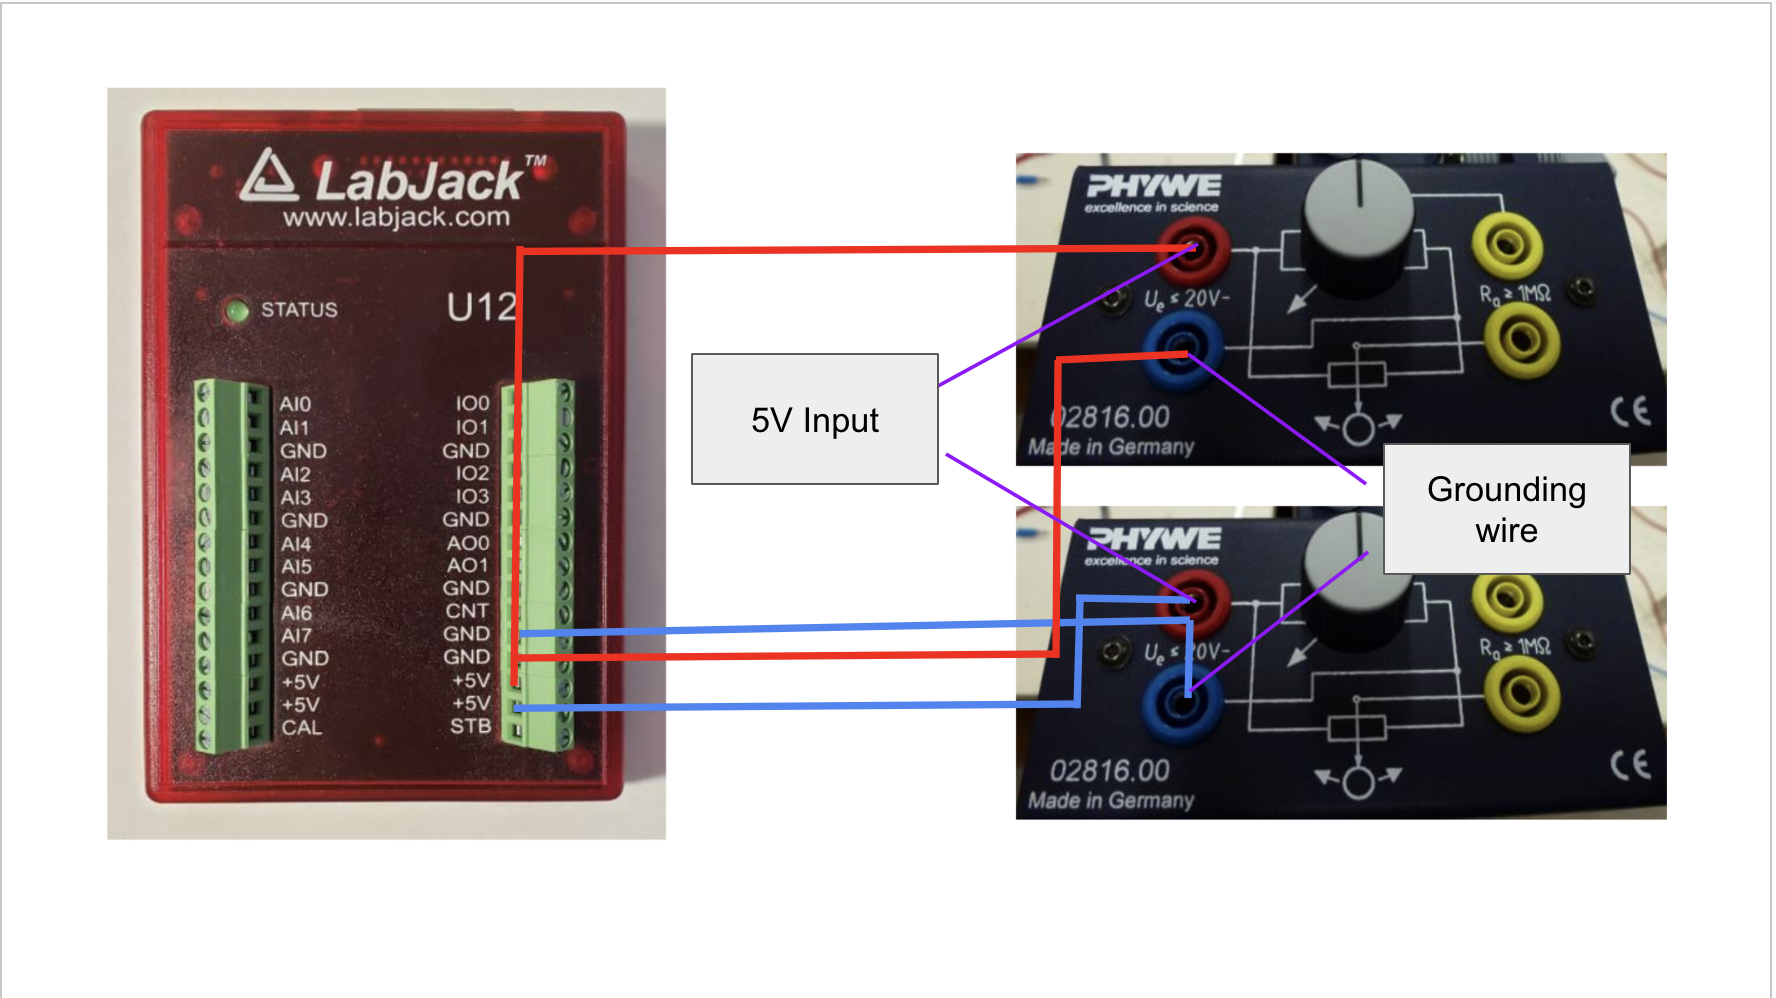
\includegraphics[width=0.8\textwidth]{circuit.png}
    \caption{Diagram showing the connections between the
    Labjack and the two pendula.}
    \label{fig:circuit}
\end{figure}

To calculate the spring constant, $k$, the following procedure
can be done with the setup shown below.

\begin{figure} [H]
    \centering
    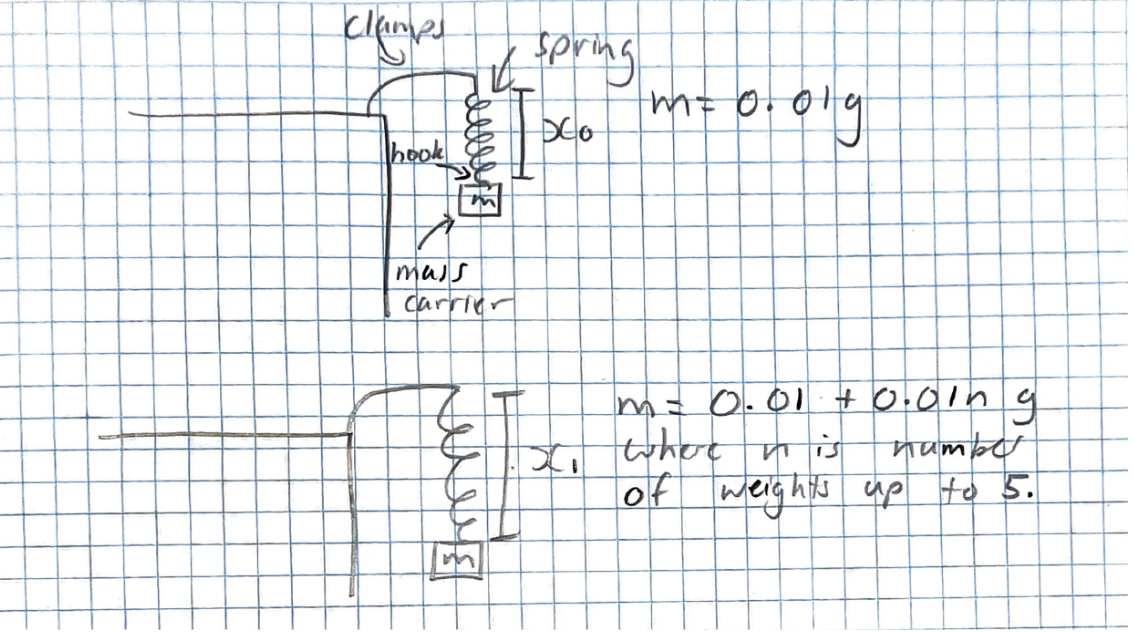
\includegraphics[width=0.8\textwidth]{k calc.png}
    \caption{Labelled diagram of setup of falling mass attached
    to spring.}
    \label{fig:k}
\end{figure}

Beginning with just the mass carrier, weighing 10g, it can be
hooked onto the spring to displace it some distance $x_0$. Once
the mass comes to rest, we can say that the net force of the mass
is zero. Since the only two forces acting on the mass are force of
the spring and the force due to gravity, we can equate the two,

\begin{equation}
    \begin{split}
        \sum F_{net} &= -mg + kx = 0 \\
        mg &= kx \\
        x &= \frac{g}{k}m.
    \end{split}
\end{equation}

By plotting a graph of spring displacement vs mass, we can take
the gradient $\frac{g}{k}$ and as $g$ is known, we can calculate k.

\section{Lab Book}
\begin{figure}[h]
    \centering
    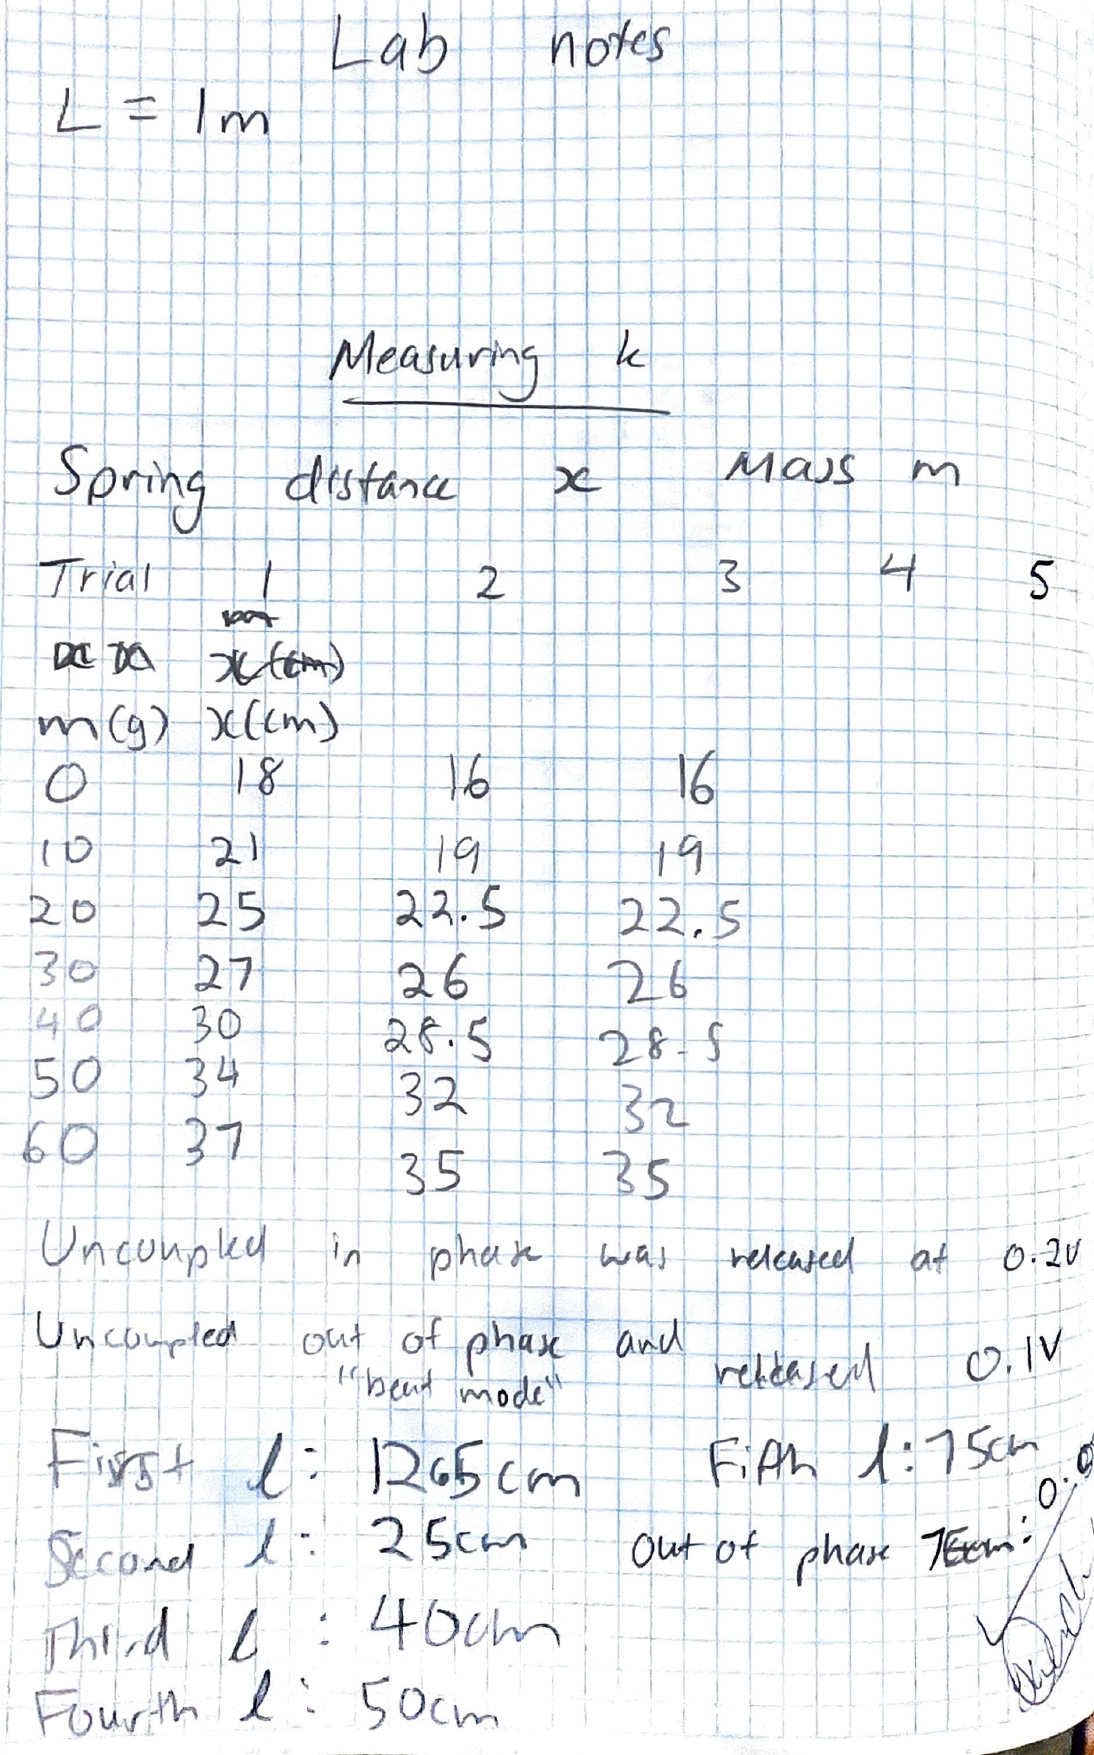
\includegraphics[width=0.8\textwidth]{labbook.jpg}
    \caption{Notes taken during the lab.}
\end{figure}


\end{document}